% ==============================================================================
% ================================== AUFGABE 6 ================================
% ==============================================================================

\section{Aufgabe 6: Datenreduktion}
\label{sec:aufgabe6}

\subsection{Methodik}

Zur Untersuchung der Datenreduktion wird ein \emph{stratifiziertes Sampling} nach der Aktion durchgeführt \texttt{train\_test\_split(stratify=\glqq action\grqq)}. Dadurch bleiben die Aktionsproportionen in jedem Subset erhalten -- ein von Géron empfohlenes Vorgehen \cite[S.~101--105]{1}. Die Verteilungstreue wird mit dem \emph{Kolmogorow-Smirnow-Test} (\ac{KS}-Test) pro Beobachtungsdimension geprüft \cite{7}. Die Nullhypothese $H_0$ lautet, dass die reduzierte Stichprobe und der Originaldatensatz aus derselben Verteilung stammen, bei einem $p$-Wert $> 0{,}05$ wird die Nullhypothese beibehalten, sodass die Verteilungen als statistisch nicht unterscheidbar gelten (Standardverfahren des KS-Tests). Zusätzlich wird für jede Reduktionsstufe (5\,\%, 10\,\%, 20\,\%, 30\,\%, 50\,\%) ein Surrogatmodell trainiert und die Test-\ac{MAE} mit dem Modell auf dem vollen Datensatz verglichen.

\subsection{Ergebnisse}

Die Aktionsverteilung im Original ist stark unbalanciert: \emph{noop}~48{,}84\,\%, \emph{main}~40{,}73\,\%, \emph{left}~5{,}31\,\%, \emph{right}~5{,}12\,\% (eigene Messung). Durch stratifiziertes Sampling bleiben die Anteile auf 0{,}1 Prozentpunkte erhalten (Tabelle~\ref{tab:a6_aktionen}). Der \ac{KS}-Test ergibt für das 10\,\%-Subset auf allen acht Beobachtungsdimensionen $p > 0{,}05$ (zwei Dimensionen sogar $p = 1{,}0$), die Nullhypothese gleicher Verteilungen kann also nicht abgelehnt werden (eigene Berechnung).

\begin{figure}[H]
    \centering
    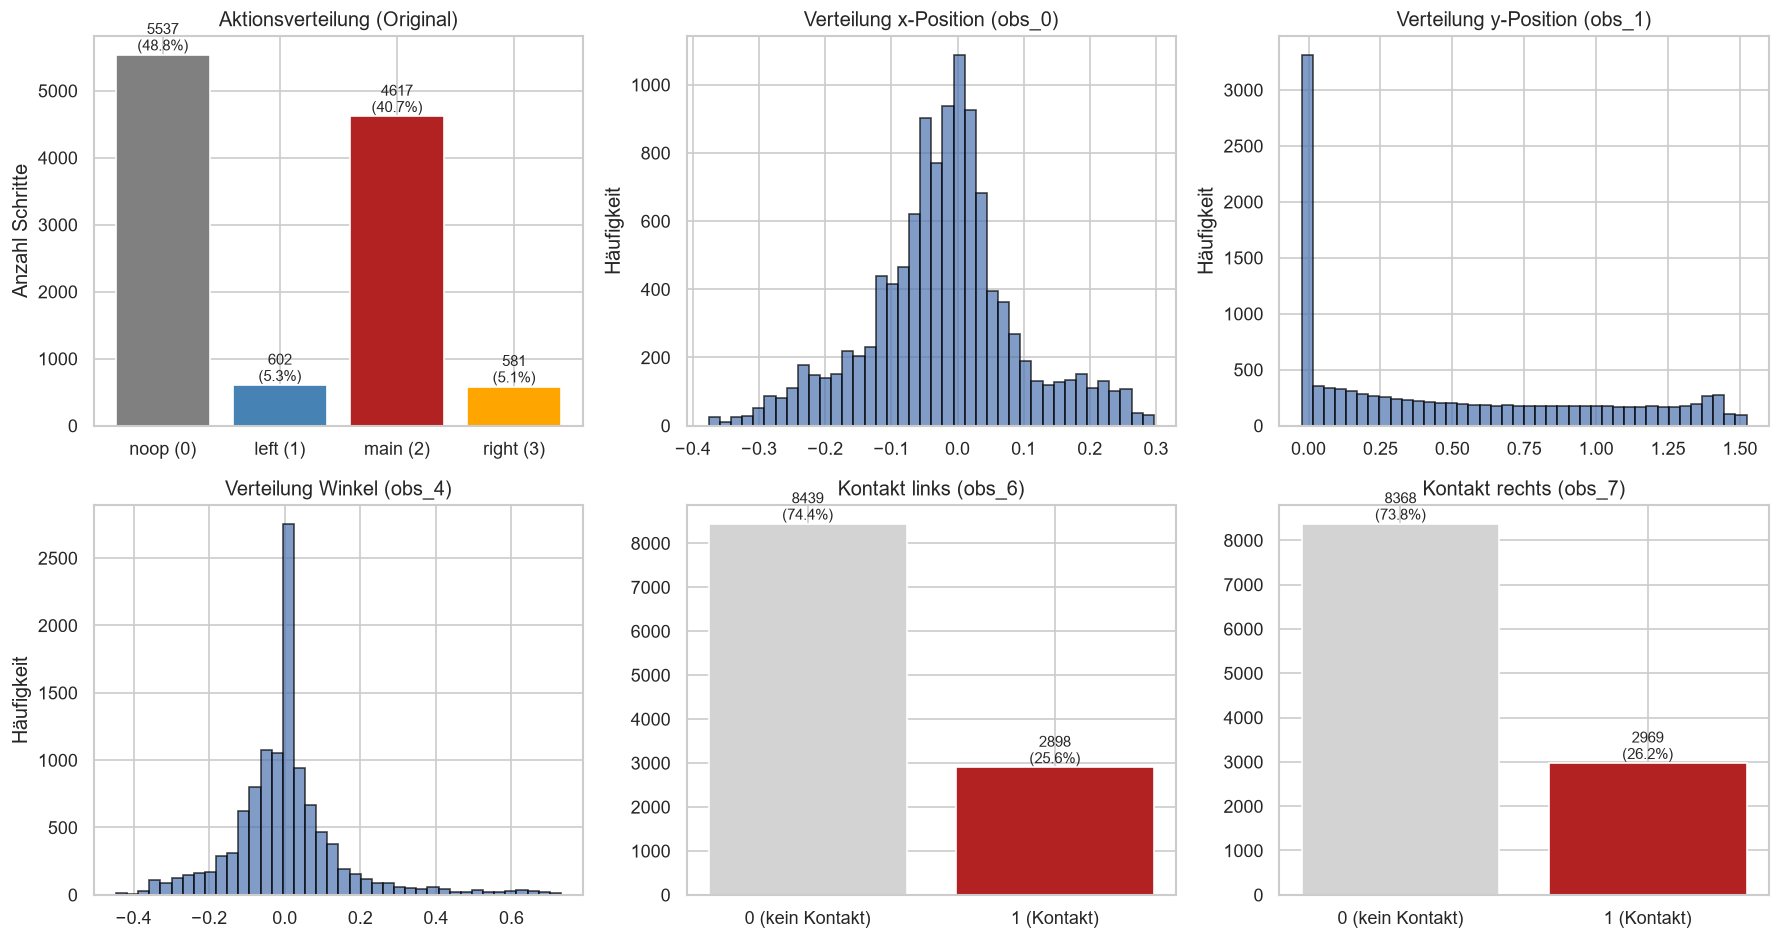
\includegraphics[width=1\linewidth]{asset/image/TomaKing_A6_Originalverteilung.png}
    \caption{Verteilung der Originaldaten \textit{(eigene Darstellung)}.}
    \label{fig:a6_orig}
\end{figure}

\begin{table}[H]
    \centering
    \begin{tabular}{lrrr}
        \toprule
        Aktion & Original & 10\,\%-Subset & 5\,\%-Subset \\
        \midrule
        \emph{noop}  & 0{,}4884 & 0{,}4885 & 0{,}4885 \\
        \emph{left}  & 0{,}0531 & 0{,}0529 & 0{,}0529 \\
        \emph{main}  & 0{,}4073 & 0{,}4074 & 0{,}4074 \\
        \emph{right} & 0{,}0512 & 0{,}0511 & 0{,}0511 \\
        \bottomrule
    \end{tabular}
    \caption{Aktionsverteilung im Original und in reduzierten Datensätzen \textit{(eigene Darstellung)}.}
    \label{tab:a6_aktionen}
\end{table}

\begin{figure}[H]
    \centering
    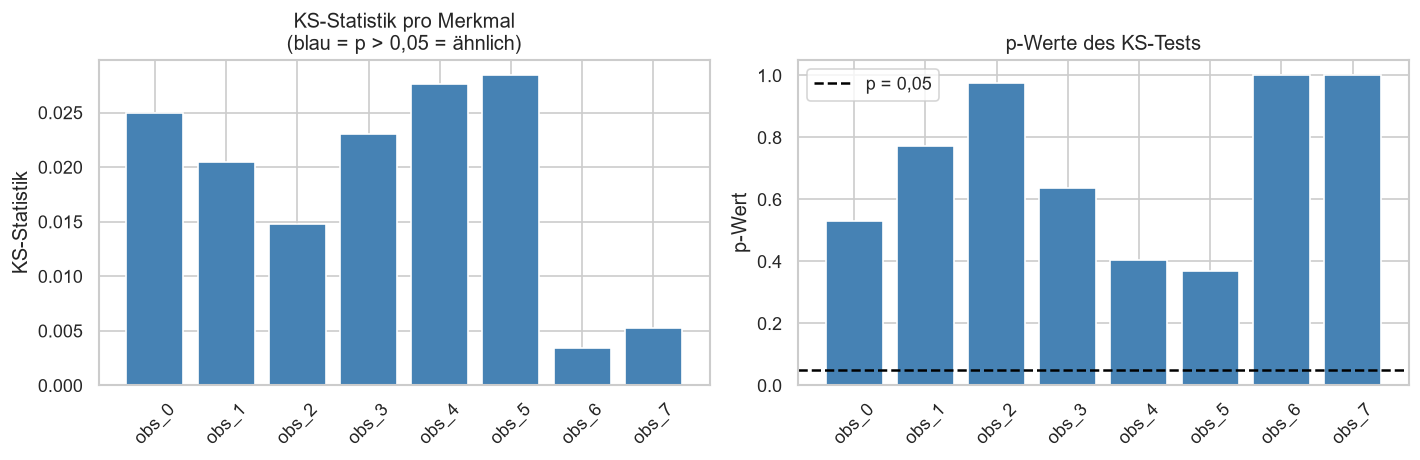
\includegraphics[width=1\linewidth]{asset/image/TomaKing_A6_KS_Test.png}
    \caption{\ac{KS}-Test: Original vs.\ 10\,\%-Subset \textit{(eigene Darstellung)}.}
    \label{fig:a6_ks}
\end{figure}

Die Modellqualität sinkt mit abnehmender Datenmenge (Tabelle~\ref{tab:a6_mae}). Während das 30\,\%-Subset noch eine Test-\ac{MAE} von $0{,}01307$ erreicht (rund 18\,\% schlechter als das Modell auf vollen Daten), verschlechtert sich die Qualität bei 10\,\% auf $0{,}01904$ (rund 72\,\% schlechter, eigene Messung).

\begin{table}[H]
    \centering
    \begin{tabular}{lrrr}
        \toprule
        Datensatz & $n_{\text{train}}$ & Test-\ac{MSE} & Test-\ac{MAE} \\
        \midrule
        Original (100\,\%)        & 7\,935 & 0{,}00184 & 0{,}01106 \\
        Stratifiziert (50\,\%)    & 3\,967 & 0{,}00118 & 0{,}01239 \\
        Stratifiziert (30\,\%)    & 2\,380 & 0{,}00124 & 0{,}01307 \\
        Stratifiziert (20\,\%)    & 1\,586 & 0{,}00148 & 0{,}01604 \\
        Stratifiziert (10\,\%)    &   793 & 0{,}00257 & 0{,}01904 \\
        Stratifiziert (5\,\%)     &   396 & 0{,}00114 & 0{,}02154 \\
        \bottomrule
    \end{tabular}
    \caption{Test-\ac{MAE} des Surrogatmodells auf unterschiedlich großen Subsets \textit{(eigene Darstellung)}.}
    \label{tab:a6_mae}
\end{table}

\begin{figure}[H]
    \centering
    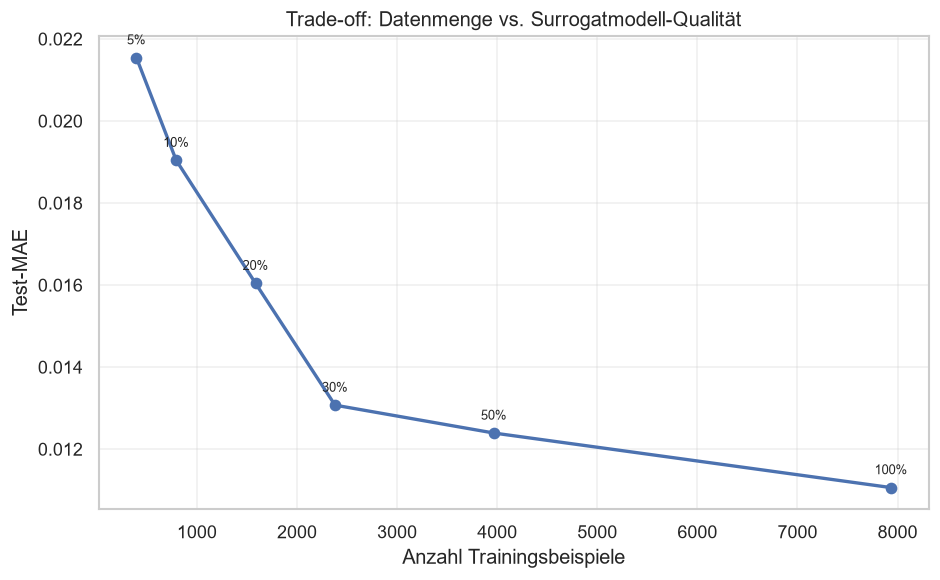
\includegraphics[width=1\linewidth]{asset/image/TomaKing_A6_Tradeoff.png}
    \caption{Trade-off zwischen Datenmenge und Test-\ac{MAE} \textit{(eigene Darstellung)}.}
    \label{fig:a6_tradeoff}
\end{figure}

\subsection{Interpretation}

Die stratifizierte Reduktion erhält die Aktionsverteilung exakt und die Verteilung der Beobachtungsdimensionen statistisch nachweisbar -- die Nullhypothese des KS-Tests kann in keiner Dimension abgelehnt werden. Dennoch verschlechtert sich die Modellqualität mit abnehmender Datenmenge, und anders als erhofft zeigt sich kein breites Plateau, auf dem die Modellgüte stabil bleibt. Der Sweet Spot liegt bei etwa 30 \% der Originaldaten: Hier sinkt die Trainingsmenge auf unter ein Drittel, während der Test-MAE nur moderat ansteigt -- ein sinnvoller Kompromiss zwischen Rechenaufwand und Modellqualität. Die nicht-monotone Entwicklung bei 5 \% gegenüber 10 \% ist auf die hohe Varianz bei sehr kleinen Datensätzen zurückzuführen \cite[S.~151--153]{1}: Bei nur 400--800 Trainingsbeispielen ist auch der Validierungsdatensatz für Early Stopping so klein, dass die Auswahl der besten Epoche unzuverlässig wird. Für die Praxis empfiehlt sich daher ein Anteil von mindestens 20--30 \% der Originaldaten.

% ==============================================================================
% ================================== AUFGABE 6 ================================
% ==============================================================================